% !TEX root = ../paper.tex

\section{Semantic Similarity Classification of Comment Usefulness}

\textbf{Definition:} We define a \emph{useful} comment as one that directly contributes to improving a proposed change, and a \emph{useless} comment as one that does not\footnote{Although we call these comments \emph{useless} in our study, it might actually have utility--or sometimes  be required---in some other contexts, such as to facilitate communication or to enforce guidelines or process.}.

Our goal here is to improve the efficiency and confidence in the task of determining the usefulness of review comments.
As with many subjective assessments, usefulness is not dichotomous and hence we must accept a third qualification, \emph{unclear}, to allow for the case where a comment does not directly make a positive contribution but is not clearly out of scope or tangential i.e. it may be useful.
Our approach is largely based on the assumption that usefulness is determined by the relevance a comment has to the proposed change (as documented within a MCR system).
A primary factor in relevance is similarly, and so it is natural for us to consider classification using \emph{similarity conditions}. 
%\cite{Davies2012}
%\dan{can we find a reference for relevance and similarly?}
We speculate that the more similar a comment is to the proposed change, the more relevant it is and hence more likely useful.
Conversely, the more dissimilar\footnote{This is technically not simply the opposite of similarity. Unlike similarity, dissimilarity can be arbitrarily large.}, the less relevant, and hence less useful.

\subsection{Approach}
We seek to develop a model based on similarity criteria to classify (i.e. \emph{determine}) comments as either useful or useless. 
Given the subjective nature of usefulness, precise classification conditions probably do not exist and so we resort to conditions that indicate a meaningful \emph{likelihood} of classification.
That is, for some degree of similarity a comment is determined to be \emph{most likely useful}, and for some degree of dissimilarity it is \emph{most likely useless}. Because this is a liklihood model, it is possible that a classification cannot be determined (i.e. no classification is likely enough) or determined to be in multiple classifications (i.e. overlap in likelihood conditions). It's important to keep in mind that these last two outcomes are not actual classifications whose interpretation is difficult and perhaps unreliable.     
The key to our approach is to determine the classification conditions in a practical, assurable manner that also is effective to use for assessing comment usefulness.

Fig. \ref{fig:overview} shows an overview of our proposed classification approach.
Usefulness of a comment is determined by computing its semantic similarity with the commit message of its proposed change and observing if it satisfies \emph{usefulness classification likelihood conditions}.
The conditions are simply threshold values of similarity and dissimilarity empirically determined to optimize a desired likelihood objectives. While more complex conditions are possible and may perform better, we begin with this simple model and investigate if it is sufficient for our assessment task.


\begin{figure}[!t]
\centering
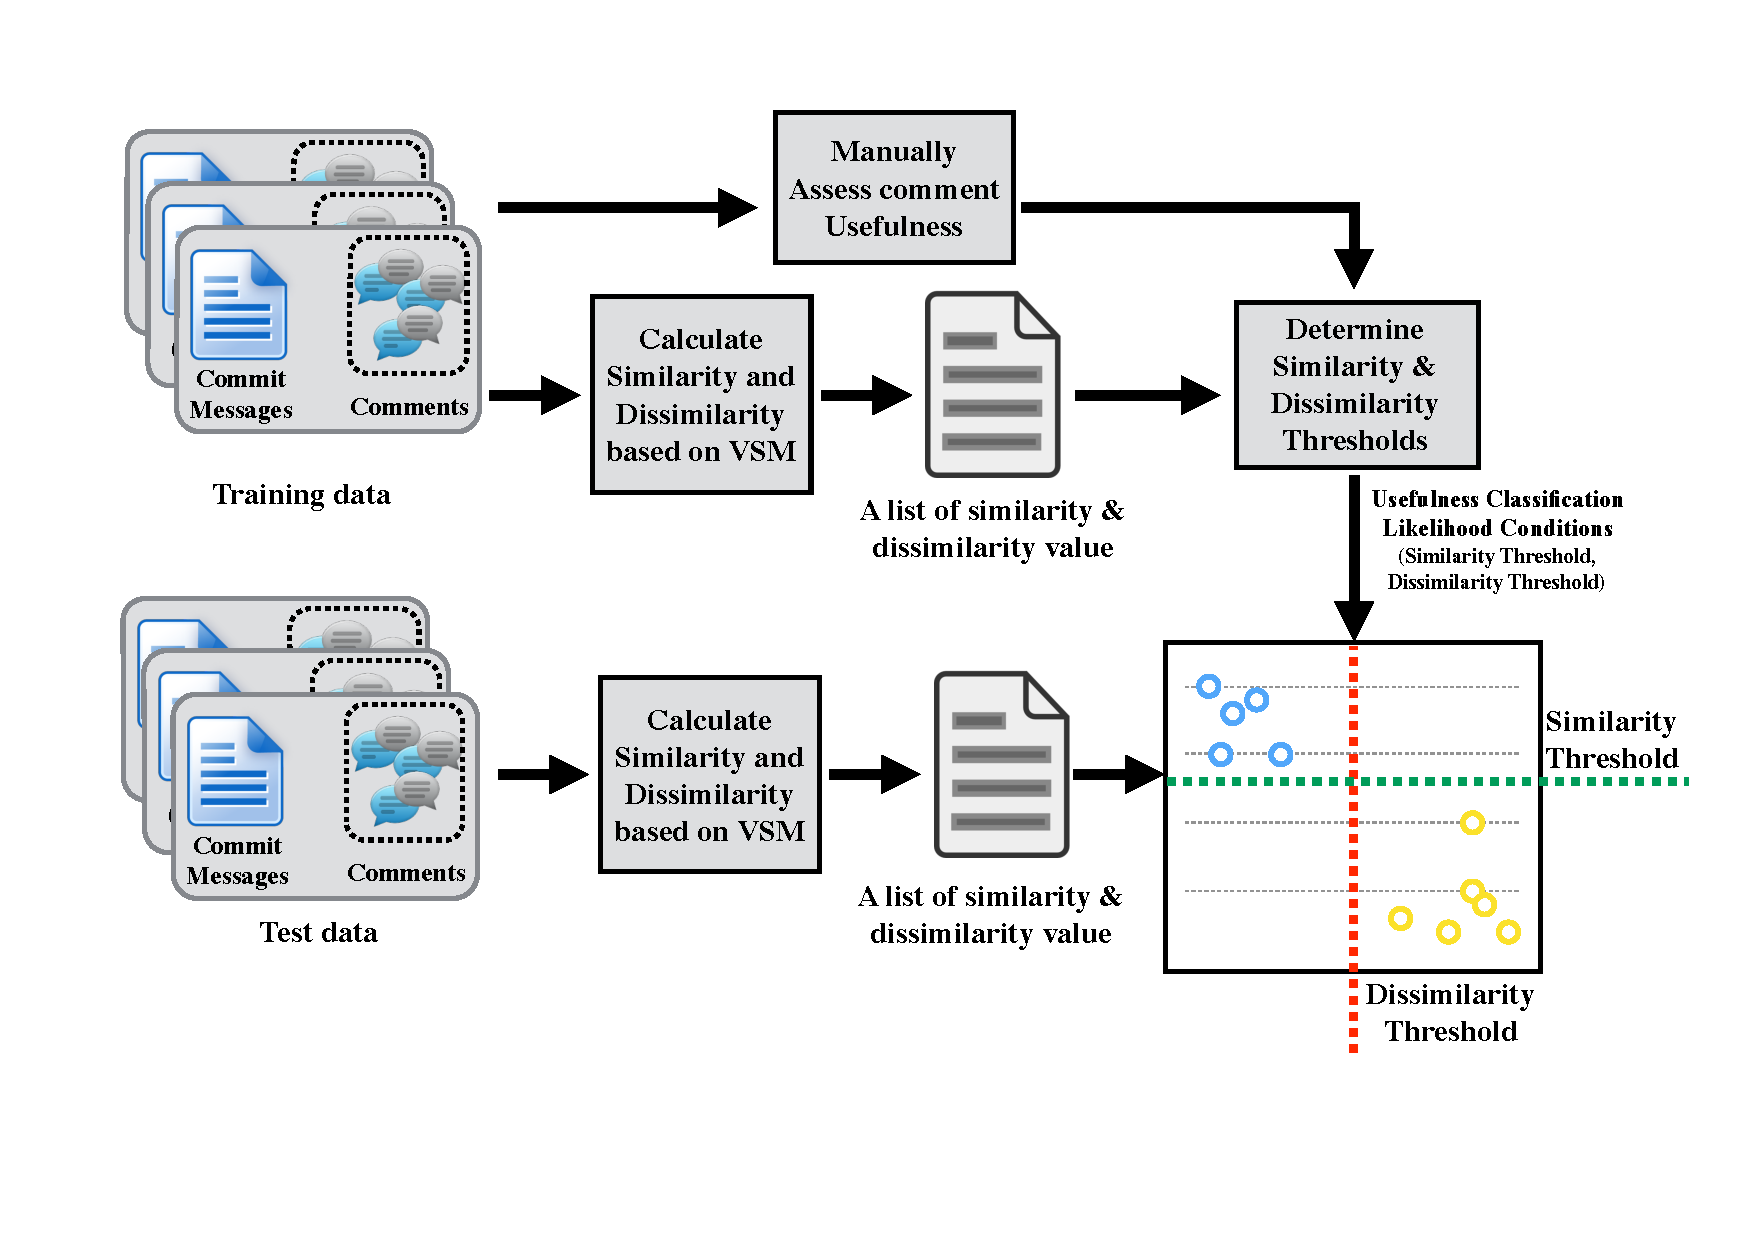
\includegraphics[scale=0.34, trim = 50 90 0 30, clip=true]{overview2}
\caption{An overview of classification of comment usefulness using semantic similarity}
\label{fig:overview}
\end{figure}

% again, I can't see Fig. \ref{fig:overview}(a)
% Thai sez: Cosine distance IS NOT cosine similarity. Cosine distance is defined as 1 - cosine similarity, and is not a proper distance metric, lacking triangle equality and stuff [Wikipedia].
We calculate semantic similarity using the Vector Space Model (VSM)% \cite{wiki:vdm}
with the cosine similarity measure, which is a well-known technique for retrieving relevant documents written in unstructured natural language. The Euclidian distance, which is a well-established measure of dissimilarity,  applies here analogously for retrieving irrelevant documents.
%For our case example training dataset, we manually identified 320 randomly-selected pairs of comments and corresponding commit messages in Fig. \ref{fig:overview}(b). \thai{The %overview figure does not have (a) and (b)...}
%\dan{what was the actual effort (in person-hours) to create the training data?}

The model is a form of \emph{supervised classification}% \cite{wiki:supervised}
where a training set is used to empirically derive similarity and dissimilarity thresholds that optimize meaningful likelihoods e.g. likelihood that a comment is useful given its similarity is greater than some threshold value.    
The training data is a small set of randomly-selected pairs of comments and the corresponding commit messages.
These comments are manually assessed for usefulness.
%Each comment is assessed by three different people independently.
%For each \texttt{YES} vote, a single point is given to that comment.
%This means that a comment will receive a score of 0, 1, 2, or 3.
For statistical purposes, at least 30 useful and 30 useless comments must be collected.
The similarity and dissimilarity metrics are then computed for the training data set.
These are used to estimate the similarity and dissimilarity thresholds $S_T$ and $D_T$ that best discriminate useful comments and $S'_T$ and $D'_T$ for useless comments. 
%Other likelihood functions could be used depending on precision, recall, or risk goals.
We find these thresholds by selecting $s_t,d_t$ values that maximize the F-measure \footnote{\url{http://en.wikipedia.org/w/index.php?title=F1_score&oldid=608940880}},
which is a performance measure for a binary classification that compromises trade-offs in accuracy of classification (precision) and coverage of classification (recall).
In this study, we used the F$_1$-measure, which equally prioritizes precision and recall.
Different weighting can be used by different F$_\beta$ measures depending on error tolerance for precision and recall.


\subsection{Usefulness Classification Model} 
Using thresholds derived from the training data as discussed above, we can classify the usefulness of comments for the entire review according to the classification model as follows: given a comment $c$ and a corresponding commit message $m$,
\begin{itemize}
\item \textbf{Useful}: $\Theta(c,m,S_T,D_T) = \True$ iff $\Sim(m,c) \geq S_T$ and $\Dist(m,c) \leq D_T$.
\item \textbf{Useless}: $\Omega(c,m,S'_T,D'_T) = \True$ iff $\Sim(m,c) \leq  S'_T$ and $\Dist(m,c) \geq D'_T$.
\item \textbf{\emph{undetermined}}: neither (no condition holds) or both (overlap of conditions) of the above conditions are $\True$.
% We also refer to them as \emph{neither} and \emph{overlap}.
\end{itemize}

The functions $\Sim(m,c)$ and $\Dist(m,c)$ are the similarity and dissimilarity measures relative to the proposed change commit message $m$ for the text of comment $c$ using cosine similarity and euclidian distance, respectively.
Two metrics are used because they are independently generated and thus provides better discrimination for classification.
We also found experimentally that using two metrics has higher performance than just one. We note again that ``undetermined" is not a meaningful classification in our model.

% The details of our approach are elaborated in the following subsections.

%\dan{**** ALERT **** this entire subsection is not needed! Everything in it is well-known and can simply be referenced. I suggest removing it if we need the space.  I have not edited this section .... }
%\subsection{Similarity and Dissimilarity Calculation based on VSM}
%%Vector Space Model (VSM) is well-known technique for information retrieval where documents written in unstructured natural language. In Software Engineering, VSM has been widely use to find relationship among documents in software issue tracking system\cite{Davies2012}.
%For each review, we compute similarity and dissimilarity of every comments comparing with the commit message which is described the purpose of the change.
%To do so, we use VSM which is a model for representing text documents as vectors.
%For a set of commit messages and comments ($D$), each document, $d$ (commit message or comment) is represented as $\overrightarrow{V_d} = <w_{1,d},w_{2,d},w_{3,d},...w_{n,d}>$, where $n$ is the total number of unique terms occur in $D$.
%The $w_{t,d}$ value is tf-idf weighting of term $t$ calculated from term occurrence frequency using Equation \ref{eq:tf-idf} where $\operatorname{tf}_{t,d}$ is frequency of term $t$ occurs in document $d$; and $|\{d' \in D | t \in d'\}|$ is the number of other documents $d'$ that also contain term $t$.  
%
%\begin{equation}
%w_{t,d} = \operatorname{tf}_{t,d} \times \log\frac{|D|}{|\{d' \in D \:|\: t \in d'\}|}
%\label{eq:tf-idf}
%\end{equation}
%
%After transforming commit message and comments to vectors, we calculate similarity using Cosine similarity and Euclidian distance. 
%
%
%\noindent\textbf{Cosine similarity} measures similarity between two vectors using inner product. Given a vector commit message $\overrightarrow{V_m}$ and the vector of its comments $\overrightarrow{V_m}$, we can calculate Cosine similarity using Equation \ref{eq:cosine}. The similarity value is ranging $[0,1]$ where 0 means there is no similarity and 1 means two vectors are textually similar.  
%
%\begin{equation}
%\Sim(c) = \cos\theta(\overrightarrow{V_m},\overrightarrow{V_c}) = \frac{\sum_{i=1}^{|D|} w_{i,m} \times w_{i,c}}{\sqrt{\sum_{i=1}^{|D|} w^2_{i,m} \times \sum_{i=1}^{|D|} w^2_{i,c}}}
%\label{eq:cosine}
%\end{equation}
%
%\noindent\textbf{Euclidian distance} measures ordinary distance between each element of two vectors using Equation \ref{eq:euclid}. We can use this distance as an dissimilarity. Given a vector commit message $\overrightarrow{V_m}$ and the vector of its comments $\overrightarrow{V_m}$, we can calculate Euclidian distance using Equation \ref{eq:cosine}. The distance value is ranging $[0,\infty)$ where 0 means these vectors are the same vectors while a more distance means these vectors are less similar.
%
%\begin{equation}
%\Dist(m,c) = \|\overrightarrow{V_m} - \overrightarrow{V_c}\| = \sqrt{\sum_{i=1}^{|D|}(w_{i,m} - w_{i,c})^2}
%\label{eq:euclid}
%\end{equation}
%
%\subsection{Estimating Similarity and Dissimilarity Thresholds}
%Suppose we use $\Theta(c,S_T=s_t,D_T=d_t)$ to classify useful comments and we have the following values:
%
%$\mathrm{TP}_{s_t,d_t}$ is the number of comments that our model classified as \textit{useful} and are \textit{actually useful} i.e. true-positives; 
%
%$\mathrm{FP}_{s_t,d_t}$ is the number of comments that our model classified as \textit{useful} but are \textit{actually useless} i.e. false positives;
%
%$\mathrm{FN}_{\theta_s,\theta_d}$ is the number of comments that our model classifies as \textit{useless} but are \textit{actually useful}. 
% 
%We can now define the following classification  performance measures: 
%\begin{equation}
%\begin{split}
%\mathrm{F\text{-}measure}_{s_t,d_t} &= 2 \times \frac{\mathrm{precision}_{s_t,d_t} \times \mathrm{recall}_{s_t,d_t}}{\mathrm{precision}_{s_t,d_t} + \mathrm{recall}_{s_t,d_t}}
%\\
%\mathrm{precision}_{s_t,d_t}  &= \frac{\mathrm{TP}_{s_t,d_t}}{\mathrm{TP}_{s_t,d_t}+\mathrm{FP}_{s_t,d_t}}
%\\
%\mathrm{recall}_{s_t,d_t}  &= \frac{\mathrm{TP}_{s_t,d_t}}{\mathrm{TP}_{s_t,d_t}+\mathrm{FN}_{s_t,d_t}}
%\end{split}
%\label{eq:fmeasure}
%\end{equation}

% Our proposed approach is empirically driven and automatically adjusts to the quality the data.
While our proposed approach is straightforward, empirically driven, and automatically adjusts to the quality of the data, it has a few drawbacks.
First, we must accept that some comments cannot be reliably or confidently classified.
We denote these as \emph{undetermined} to differentiate them from comments whose usefulness is \emph{unclear} (i.e. cannot be subjectively assessed as useful or useless).
Secondly, owing to the subjective assessment of usefulness and our need to represent this, not just any classification, this fundamentally implies performing supervised classification requiring nontrivial training data to define representative classification sets.


% empirically driven and automatically adapts to the quality the data


% Thai sez: We did not mention the F-measure for \Theta, thus suddenly referring to \Omega does not make much sense...
% The F-measure for $\Omega(c,S_T=s_t,D_T=d_t)$ is computed analogously where we change instances of useful to useless and vice-versa in the definitions. The correctness of classification is determined from the useful/useless defined dataset. 


%Using this method, we iteratively measure an accuracy for values of $s_t$ and $s'_t$ ranging $[0,1]$; and values of $d_t$ and $d'_t$ ranging $[0,\infty)$. 

%\begin{equation}
%\mathrm{F\text{-}measure}_{S_T,D_T} = \frac{2\mathrm{TP}_{S_T,D_T}}{2\mathrm{TP}_{S_T,D_T}+\mathrm{FP}_{S_T,D_T}+\mathrm{FN}_{S_T,D_T}}
%\label{eq:precision}
%\end{equation}

%where $\mathrm{TP}_{S_T,D_T}= |\{ c \in C |  \text{\textbf{useful}}(c,S_T,D_T) = \mathrm{TRUE} \}\cap \{c \in C| \mathrm{vote}(c) = 2\}|$,  $\mathrm{FP}_{S_T,D_T} = |\{ c \in C | \text{\textbf{useful}}(c,S_T,D_T) = \mathrm{FALSE} \}\cap \{\mathrm{vote}(c) = 2\} $, $\mathrm{FN}_{S_T,D_T} = |\{ c | c \in C, \text{\textbf{useful}}(c,S_T,D_T) = \mathrm{TRUE} \}\cap \{\mathrm{vote}(c) < 2\} $
%According to this, we can formalize as follows:

%\begin{equation}
%(S_T,D_T) = \max(\{\mathrm{F\text{-}measure} \text{ of \textbf{useful}}(c,s_T,d_T) | s_T\in[0,1] \text{ and } d_T\in [0,\infty) \})
%\end{equation}
